\documentclass{jarticle}

\setlength{\voffset}{-65pt}
\setlength{\oddsidemargin}{-5mm}
\setlength{\textwidth}{490pt}
\setlength{\textheight}{700pt}

\usepackage{graphicx}
\usepackage{amsmath,amssymb,pifont,colortbl,amscd, wrapfig, ascmac}
\usepackage{amsthm}
\usepackage{url}
\usepackage{bm}

\newtheorem{theorem}{定理}
\newtheorem{definition}{定義}
\newtheorem{example}{例}

\def\ev{\mathrm{ev}}
\def\c{\mathop{\mathrm{cts}}\nolimits}
\def\odd{\mathop{\mathrm{odd}}\nolimits}
\def\diag{\mathop{\mathrm{diag}}\nolimits}
\def\mod{\mathop{\mathrm{mod}}\nolimits}
\def\deg{\mathop{\mathrm{deg}}\nolimits}
\def\inv{\mathop{\mathrm{Inv}}\nolimits}
\def\cl{\mathop{\mathrm{cl}}\nolimits}
\def\ad{\mathop{\mathrm{ad}}\nolimits}
\newcommand{\sad}{\overline{\ad}}
\def\tr{\mathop{\mathrm{tr}}\nolimits}
\def\End{\mathop{\mathrm{End}}\nolimits}
\def\id{\mathop{\mathrm{id}}\nolimits}
\def\ev{\mathop{\mathrm{ev}}\nolimits}
\def\coev{\mathop{\mathrm{coev}}\nolimits}
\def\coad{\mathop{\mathrm{coad}}\nolimits}
\def\Ob{\mathop{\mathrm{Ob}}\nolimits}
\def\Hom{\mathop{\mathrm{Hom}}\nolimits}
\def\im{\mathop{\mathrm{Im}}\nolimits}
\def\Span{\mathop{\mathrm{Span}}\nolimits}
\def\ideal{\mathop{\mathrm{ideal}}\nolimits}
\def\co{\colon\thinspace}
%for U_h
\newcommand{\uqenh}[1]{ (\bar U_q^{\ev})\,\hat  {}^{\;\hat  \otimes #1}}
\newcommand{\uqen}[1]{ (\bar U_q^{\ev})\;\tilde {}^{\;\tilde \otimes #1}}
\newcommand{\uqe}{\bar U_q^{\ev}}
\newcommand{\uqz}{\bar U_q^0}
\newcommand{\uqze}{\bar U_q^{\ev 0}}
\newcommand{\uq}{\bar U_q}
\newcommand{\muq}{\mathcal{ U}_q}
\newcommand{\muqe}{\mathcal{ U}_q^{\ev}}
\newcommand{\uqzq}{U_{\mathbb{Z},q}}
\newcommand{\uqzqe}{(U_{\mathbb{Z},q})^{\ev}}
\newcommand{\uqn}[1]{\bar U_q^{\otimes {#1}}}
\newcommand{\uhn}[1]{\bar U_h^{\hat \otimes {#1}}}
\newcommand{\f}[1]{\tilde F^{({#1})}}
\newcommand{\e}[1]{\tilde E^{({#1})}}
\newcommand{\Z}{\mathbb{Z}[q,q^{-1}]}
\def\ZA{\mathbb{P}^{\mathrm{fin}}\big( \Hom_{\mathcal{A}}(0,g)\big)}

\def\deg{\mathop{\mathrm{deg}}\nolimits}
\def\inv{\mathop{\mathrm{Inv}}\nolimits}
\def\cl{\mathop{\mathrm{cl}}\nolimits}
\def\ad{\mathop{\mathrm{ad}}\nolimits}
\def\tr{\mathop{\mathrm{tr}}\nolimits}
\def\End{\mathop{\mathrm{End}}\nolimits}
\def\id{\mathop{\mathrm{id}}\nolimits}
\def\ev{\mathop{\mathrm{ev}}\nolimits}
\def\coev{\mathop{\mathrm{coev}}\nolimits}
\def\coad{\mathop{\mathrm{coad}}\nolimits}
\def\Ob{\mathop{\mathrm{Ob}}\nolimits}
\def\Hom{\mathop{\mathrm{Hom}}\nolimits}
\def\Sets{\mathop{\mathrm{Sets}}\nolimits}
\def\im{\mathop{\mathrm{Im}}\nolimits}
\def\co{\colon\thinspace}

%%% ywr extend 
\def\d{\mathrm d}
\def\grad{\mathrm grad}
\def\rot{\mathrm{\bm rot}}
\def\div{\mathrm{div}}
%%%

\begin{document}

\title{微分積分続論(ベクトル解析)} 
\author{鈴木 咲衣}
\date{平成27年度前期}
\maketitle

\begin{center} {\Large 演習問題9 } \end{center}
\begin{enumerate}
\item \cite[章末問題2.9]{koba}
曲面$(3 \sin \theta \cos \varphi, 2sin \theta \sin \varphi, \cos \theta )$, $0\leq \theta \leq \pi, 0\leq \varphi \leq 2\pi$, を考える.
\begin{enumerate}
\item この曲線の概形を描け.
\item $\theta=\frac{\pi}{3}, \varphi=\frac{\pi}{4}$における点での単位法線ベクトルを求めよ.
\end{enumerate} 
\item \cite[問題2.48]{koba} 
曲面$\bm r(s,t)=(s,t, e^{s-t})$の上の点$\bm r(1,0)$においての接平面の式を求めよ.
\item \cite[問題7.12]{koba} 
次のベクトル場$\bm V$の回転を求め,さらに原点において,\underline{単位ベクトル$\bm u$の方向を軸とする回転}を求めよ.
\begin{enumerate}
\item $\bm V=(y+z, xz, x^{2y}), \quad \bm u=(\frac{1}{\sqrt {2}}, \frac{1}{\sqrt {2}}, 0)$,
\item$\bm V=(\sin x+\sin z, \cos y+z\cos x, x\sin z), \quad \bm u=(\frac{1}{\sqrt {2}}, \frac{1}{\sqrt {2}}, 0)$,
\item $\bm V=(e^{-y}, e^{-z}, e^{-x}), \quad \bm u=(\frac{1}{\sqrt {3}}, \frac{1}{\sqrt {3}}, \frac{1}{\sqrt {3}})$.
\end{enumerate} 
%\item \cite[問題7.13]{koba} 

\item \cite[問題8.16]{koba} 
球面$x^{2}+y^{2}+z^{2}=1$の$z\geq 0$の部分を$\Sigma$とし,$\bm V=(y, 0, x^{2}+z^{2})$とする.このとき$\int_{\Sigma}\mathrm{rot} \bm V \cdot d\bm S$を求めよ.
ただし$\Sigma$の表は$x^{2}+y^{2}+z^{2}>1$の側とする.
\item \cite[章末問題8.9]{koba} 
回転放物面$z=x^{2}+y^{2}$の$z\leq 1$の部分を$\Sigma$とし,領域$\{(x,y,z) \ | \ z<  x^{2}+y^{2}\}$の方を表とする.
このときベクトル場$\bm V=(-y+z, xz, e^{x})$に対して$\int_{\Sigma} \mathrm{rot} \bm V \cdot d\bm S$を求めよ.
\end{enumerate}
\newpage

\begin{center} {\Large 演習問題9 解答} \end{center}
  \begin{enumerate}
    \item
      \begin{enumerate}
        \item
          (次ページを参照)
          \begin{figure}[p]
            \begin{center}
              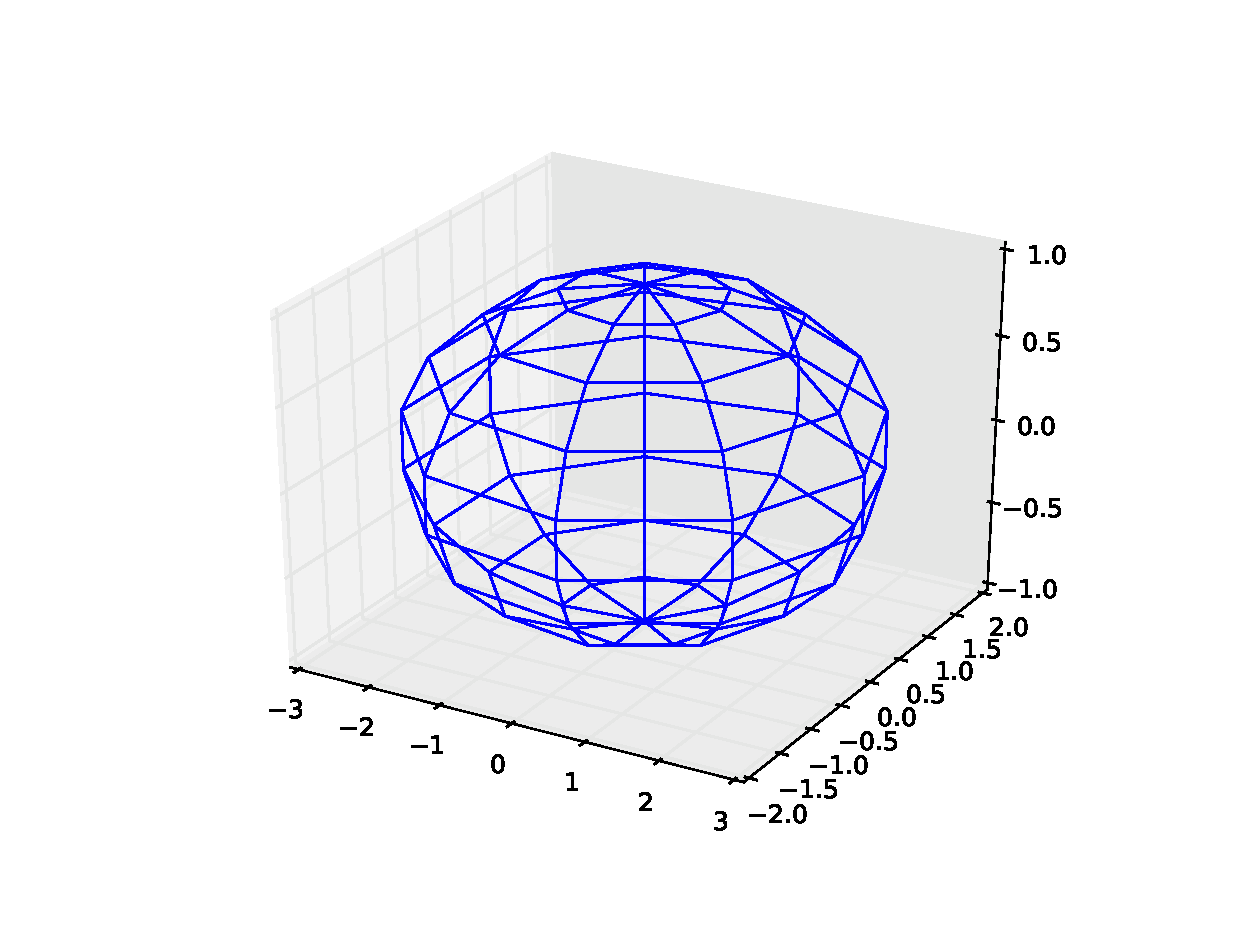
\includegraphics{answer_9_1_a.eps}
            \end{center}
          \end{figure}
        \item
      \end{enumerate}
    \item
      $\frac{\partial \bm r}{\partial s} = (1,0,e^{s-t})$かつ$\frac{\partial \bm r}{\partial t} = (0,1,-e^{s-t})$であるから、$(s,t)$における法線ベクトルは$(-e^{s-t},e^{s-t},1)$となる。よって$(1,0)$おける法線ベクトルは$(-e,e,1)$である。また${\bm r}(1,0) = (1,0,e)$から、求めるべき接平面の式は、
      \[ -e(x-1)+ey+(z-e)=-ex+ey+z=0 \]
    \item
      \begin{enumerate}
        \item
        \item
          \[\nabla \times {\bm V} = (-\cos x, \cos z - \sin z, -z\sin x)\]
          単位ベクトル$\bm u$の方向を軸とする回転は$\frac{1}{\sqrt 2}( -\cos x+\cos z -\sin z)$よって原点におけるそれは$0$となる。
        \item
          \[\nabla \times {\bm V} = (e^{-z},e^{-x},e^{-y})\]
          単位ベクトル$\bm u$の方向を軸とする回転は$\frac{1}{\sqrt 3}(e^{-z}+e^{-x}+e^{-y})$よって原点におけるそれは$\sqrt{3}$となる。
      \end{enumerate}
    \item
      $C$を$xy$平面に含まれる原点を中心とした半径$1$の円とする。また$C$の回転方向は反時計周りとする。
      \begin{eqnarray*}
        \int_\Sigma \rot {\bm V} \cdot \d {\bm S} & = & \int_C {\bm V} \cdot \d {\bm r} \\
        & = & \int_C y \d x = \int_0^{2\pi} \sin^2 \theta \d \theta = \pi
      \end{eqnarray*}
    \item
     $C$を$z=1$平面に含まれる$(0,0,1)$を中心とした半径$1$の円とする。また$C$の回転方向は反時計周りとする。
      \begin{eqnarray*}
        \int_\Sigma \rot {\bm V} \cdot \d {\bm S} & = & - \int_C {\bm V} \cdot \d {\bm r} = - \int_C (-y+1) \d x + x \d y \\
        & = & - \int_C -y \d x + x \d y = - 2 \pi
      \end{eqnarray*}
  \end{enumerate}
\end{document}